\section {Introduction}
\label{sec:introduction}

%The success of the Mu2e experiment at FNAL critically depends on the ability to store, process, simulate, and analyze data in an efficient and timely way. This document describes the Offline Computing Model developed by Mu2e to accomplish these goals, striving to use efficiently all available resources while minimizing personnel and hardware needs. As HEP computing evolves rapidly, this document focuses on tools and systems rather than specific algorithms and products. This strategy enables the development of flexible solutions that can be quickly adapted to an ever-changing computing landscape, taking full advantage of new technologies or facilities as they emerge.

The success of the Mu2e experiment at FNAL critically depends on the ability to store, process, simulate, and analyze data in an efficient and timely way. This document presents the Offline Computing Model (OCM) developed by Mu2e to accomplish these goals. It describes the software, infrastructure, tools, and workflows to perform the various computing tasks throughout the life of the experiment. In the following, Offline covers all computing activities besides the data acquisition system and the trigger software. 

The Computing Model strives to use efficiently all available resources while minimizing personnel and hardware needs. As HEP computing evolves rapidly, this document focuses on tools and systems rather than specific algorithms and products. This strategy enables the development of flexible solutions that can be quickly adapted to an ever-changing computing landscape, taking full advantage of new technologies or facilities as they emerge. This document begins by a brief introduction of the Mu2e experiment and the challenges faced by Offline computing, followed by an overview of the Computing Model and a detailed description of each of its components.

\subsection {The Mu2e Experiment}
The Mu2e experiment~\cite{TDR} aims to search for neutrino-less conversion of a negative muon into an electron in the field of a nucleus, a charged lepton flavor violating (CLFV) process. Unlike flavor violation in the quark and neutral lepton sectors, CLFV reactions are extremely suppressed in the Standard Mode (SM)~\cite{Petcov:1976ff, Marciano:1977wx, Lee:1977qz, Lee:1977tib, Blackstone:2019njl}, and an observation would be a clear sign of New Physics (see for example Ref.~\cite{Calibbi:2017uvl}). More broadly, CLFV processes are linked to the questions of flavor, families, neutrino masses, and even the matter excess of the Universe, should it arise from leptogenesis~\cite{Fukugita:1986hr, Davidson:2008bu}. 

Muon-to-electron conversion is one of the most sensitive CLFV probes in the muon sector. The best experimental limit on the process rate 
$$R_{\mu e} = \frac{\Gamma(\mu^- +N(A,Z) \rightarrow  e^- + N(A,Z))}{\Gamma(\mu^- +N(A,Z) \rightarrow \nu_\mu + N(A,Z-1))}  < 7 \times 10^{-13} \rm \, (90\% CL)$$
has been set by the SINDRUM-II experiment~\cite{SINDRUMII:2006dvw}. Mu2e plans to increase the sensitivity by four orders of magnitude using a concept developed to overcome the limitations faced by the previous generation of experiments~\cite{Dzhilkibaev:1989zb}, as illustrated in Figure~\ref{fig:Mu2eExp}. A primary $8 \GeV$ proton beam is extracted from the Fermilab Delivery Ring via slow resonant extraction~\cite{PhysRevAccelBeams.22.043501} with a pulsed timing structure of 250 ns-wide proton pulses separated by 1695 ns. The beam collides with a production target positioned at the center of the production solenoid (PS), and the pions produced in these interactions are directed towards the transport solenoid (TS) by the graded PS magnetic field. Muons are mostly formed in $\pi \rightarrow \mu \nu$ decays in the PS and TS. A target made of Al annular foils is positioned in the detector solenoid (DS), stopping about $3\times 10^{10}$ muons/s.  
In addition to pions, the primary proton beam also produces a large number of electrons, resulting in a flash of low-momentum particles reaching the detector after 150-200 ns of the primary proton interaction.
%
\begin{figure}[ht!]
\begin{center}
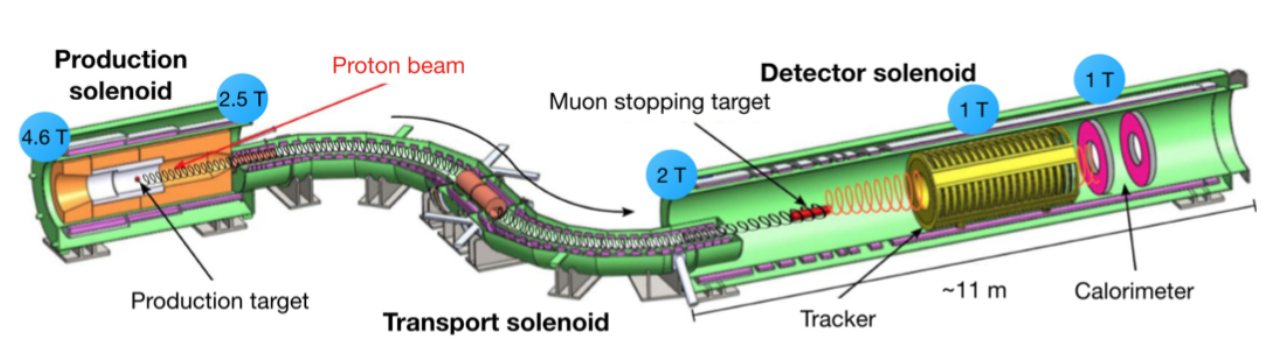
\includegraphics[width=0.9\linewidth]{figures/Mu2eExp.png}
\caption{Schematic view of the Mu2e experiment.}
\label{fig:Mu2eExp}
\end{center}
\end{figure}
%
Muons trapped in the field of the target nucleus quickly cascade down to the muonic 1s bound state before undergoing one of the following processes: neutrinoless conversion $\mu^- +N(A,Z) \rightarrow  e^- + N(A,Z)$, a coherent process resulting in the emission of a mono-energetic electron; decay in orbit (DIO) $\mu^- \rightarrow e^- \bar\nu_e \nu_\mu$, producing electrons with a momentum spectrum extending up to the conversion energy; or muon capture $\mu^- +N(A,Z) \rightarrow $ all captures, producing a wide range of final states. The conversion energy and the relative capture and decay rates depend on the nucleus. In aluminum, the capture (decay) rate is 61\% (39\%). The conversion energy is given by $E_{\mu e} = m_\mu - E_{binding} - E_{recoil} = 104.97 \MeV$, where $m_\mu$ is the muon rest mass, $E_{binding}$ denotes the binding energy in the 1s state, and $E_{recoil}$ is the nuclear recoil energy~\cite{Czarnecki:2011mx,Szafron:2017guu}. The time distribution of $\mu-e$ conversion is a function of the muonic atom lifetime ($\tau_N$), which is also nucleus-dependent. For instance, $\tau_{Al}=864$~ns and $\tau_{Au} = 74$~ns. 

Background can arise from several processes, scaling with the number of protons on target or exposure. Decays in orbit (DIO) produce a momentum spectrum extending up to the conversion energy with a rapid fall near the spectrum endpoint. Radiative pion captures $\pi^- N \rightarrow \gamma N'$ (RPC), followed by internal or external photon conversion, can also produce electrons having energies compatible with a conversion signal. This background is rejected by taking advantage of the pulsed proton beam. Since the pion lifetime (26 ns) is much shorter than the Al muonic atom lifetime (864 ns), restricting the conversion search to a time window greater than 700 ns reduces the RPC background to acceptable levels, as schematically shown in Figure~\ref{fig:Mu2ePulse}. This technique requires a beam extinction between proton pulses at the level of $10^{-10}$ to ensure that no significant amount of delayed pions are produced. Cosmic rays interacting or decaying in the detector volume are another source of background electrons, as well as antiprotons annihilating in the stopping target or the TS, beam electrons with momentum $\sim 100 \MeV$, or decays in flight of negative muons and pions in the DS. 
%
\begin{figure}[ht!]
\begin{center}
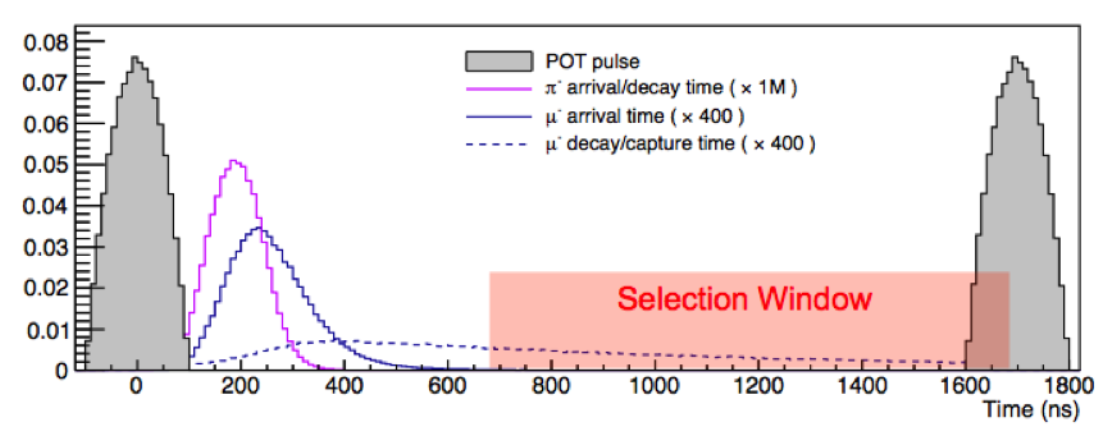
\includegraphics[width=0.9\linewidth]{figures/Mu2ePulse.png}
\caption{Proton pulses hit the production target 1695 ns apart. A delayed livegate selection window (indicated in red) is used to remove prompt backgrounds.}
\label{fig:Mu2ePulse}
\end{center}
\end{figure}
%
The detector is optimized to search for the conversion process while maintaining an expected background level below a single event. An annular tracker of approximately 3 m long containing 18 tracking stations composed of 5 mm diameter straw tubes (for a total of 20736 straws) located downstream of the stopping target. Each straw is read out from both ends, providing an estimate of the location of each hit along the wire by comparing the signal arrival times. The intrinsic momentum resolution is at the level of $\Delta p < 300 \keV$ for $100 \MeV$ electrons. An electromagnetic calorimeter comprising two annular disks containing 674 undoped CsI crystals each is positioned right after the tracker. Each disk contains 674 undoped CsI crystals read out by two silicon photo-multipliers. Test of an early prototype indicates an energy resolution $\Delta E/E \sim 16\%$ at $100 \MeV$ and a time resolution of about 100 ps~\cite{Atanova:2017ppl}. The inner regions of both detectors are left uninstrumented, blinding the apparatus to nearly all low-momentum muonic atom backgrounds and remnant beam particles. Combined measurements in the tracker and calorimeter provide particle identification sufficient to reject the background from muons misidentified as electrons. Cosmic rays interacting with the detector could produce signal-like electrons in the detector, and a Cosmic Ray Veto (CRV) system surrounding the DS and part of the TS is employed to reject this background with an efficiency of 99.99\%. It consists of modules of four layers of extruded plastic scintillation counters outfitted with wavelength-shifting fibers and read out by SiPMs. The proton beam extinction is monitored with a magnetic spectrometer built from Si pixel sensors designed by ATLAS, located downstream of the proton beam. The stopped muon rate is estimated by measuring photons emitted during the capture process with high-purity Ge and LaBr$_3$ detectors positioned in a shielding house $\sim 34$ m downstream of the stopping target foils. The data collected by each sub-system are digitized by the front-end electronics and recorded by the data acquisition system. The detector readout starts only after the flux of beam flash particles has subsided (about 500 ns after the primary proton beam hits the production target) to limit the readout rate. 

The conversion signal is identified using information from the tracker and the calorimeter. The track reconstruction algorithm is factorized into three main parts. Hits along the tracker wires are first reconstructed from the digitized signals, and a multivariate classifier is used to reject hits produced by low-momentum Compton electrons. Pattern recognition algorithms are then used to select groups of hits compatible with helical trajectories. Two separate methods are used: a calorimeter-seeded and a tracker-seeded algorithm. Finally, a Kalman fit is performed to increase the accuracy of the reconstructed track and further reject spurious candidates. The resulting efficiency for conversion electrons is around 98\% for a nominal proton bunch intensity with a background rejection factor greater than 1000. Applications of AI/ML algorithms are investigated to further improve the performance of reconstruction algorithms.

The Mu2e data-taking plan assumes two running periods (Run I and II) separated by a shutdown to upgrade the accelerator complex. The experiment will start taking data using a low-intensity proton beam to facilitate the commissioning phase before switching to a high-intensity mode. A detailed study of the various background sources has concluded that the expected Run I $5\sigma$ discovery sensitivity is $R_{\mu e} =  1.2 \times 10^{-15}$, with a total expected background of $0.11 \pm 0.03$ events~\cite{Mu2e:2022ggl}. Mu2e can also provide complementary information regarding the nature of neutrinos by searching for $\mu^- + N(A,Z) \rightarrow e^+ + N(A,Z-2)$, and search a light neutral invisible particle in $\mu^+ \rightarrow e^+ + X$ (e.g. an axion-like particle (ALP) or a familon with lepton-flavor violating couplings).
%Mu2e can also provide complementary information regarding the nature of neutrinos by searching for $\mu^- + N(A,Z) \rightarrow e^+ + N(A,Z-2)$. This reaction violates both lepton flavor conservation and lepton number conservation and could suggest the presence of non-zero Majorana neutrino masses via the “Black Box Theorem”~\cite{PhysRevD.25.2951}. 
%The experimental signature of $\mu^- + N(A,Z) \rightarrow e^+ + N(A,Z-2)$ conversion consists of a monochromatic positron of $92.3 \MeV$ for an aluminum target (assuming the daughter nucleus is in the ground state). Positrons produced from photon conversions in radiative muon captures $\mu^- + N(A,Z) \rightarrow N(A,Z-1) + \nu + \gamma(\rightarrow e^+e^-)$, represents a major background for this channel. Mu2e could also search for a light neutral invisible particle (e.g. an axion-like particle (ALP) or a familon with lepton-flavor violating couplings) in $\mu^- \rightarrow e^- + X$.

\subsection {Beam structure and run types}
The Fermilab accelerator complex will deliver the proton beam to Mu2e. As this system provides beam for other experiments as well, only a fraction of the running time will be allocated to Mu2e. Protons are first accelerated to 8 GeV and compressed into batches in the Booster Synchrotron ring. The booster can deliver proton batches every 67 ms, a time interval called a "tick". In low-intensity mode (aka 1 booster batch mode), one batch is sent to the recycler ring and re-bunched into four bunches (or spills) of $10^{12}$ protons each. The spills are then transferred to the delivery ring every 112.3 ms. The total time to perform these operations corresponds to 8 ticks. The next 12 ticks are used for accelerating beam with the main injector (MI) and delivering protons to other experiments. This 20 ticks cycle, the main injector cycle, repeats without a break for about a minute, followed by a brief pause to execute other cycles (e.g. delivering protons to the Fermilab test beam areas). This whole process is called a supercycle and is repeated uninterrupted during continuous operation. 

Each spill in the deliver ring is resonantly extracted to the Mu2e experiment. Pulses of $1.6\times 10^{7}$ protons (on average) are sent to the Mu2e primary target every 1695 ns during 107.3 ms, followed by a 5 ms reset period. This corresponds to 63 298 proton pulses per spill. The pulses are about 250 ns wide, and the number of protons between pulses is required to be less than $10^{-10}$ \cite{beamreqs} to reduce backgrounds from late interactions. In high-intensity mode (aka 2 booster batches mode), the main injector cycles are re-arranged into 21 ticks with two booster batches used to create 8 spills for Mu2e. Each spill is extracted in the delivery ring during 48.1 ms with $3.9\times 10^{7}$ protons / pulse. Including reset time, beam is sent to Mu2e for 380 ms every 1.4 ms. The low- and high-intensity beam patterns are illustrated in Figure~\ref{fig:beam}. The period during which beam is delivered to Mu2e is traditionally called "on-spill", by contrast to the "off-spill" time during which no protons are delivered. The proton bunch intensity (PBI), defined as the number of protons per pulse, can vary substantially within a spill. Slow-extraction fluctuations impart an approximately log-normal distribution on the proton pulse intensity, varying on a timescale of milliseconds. The beam intensity distribution is characterized by the Spill Duty Factor (SDF), which measures the relative spread of the proton intensity distribution. Maintaining high DAQ and reconstruction efficiency requires an SDF of at least 60\% \cite{beamreqs}.

%\red{remove if we promote DAQ into a chapter}
%The data collected by Mu2e will be labelled by a three-part identifier: run, subrun, and event. The Mu2e DAQ system (see Appendix~\ref{sec:daq}) has been designed to provide deadtimelsss transitions between subruns, while transitions between runs incur a deadtime of a few minutes to prophylactically restart processes and reload the firmware. The subrun duration is chosen so that conditions are constant throughout the subrun, it spans an integer of MI cycles, and it starts near the end of the $\sim 1$s off-spill period. Subruns will therefore contain both on-spill and off-spill data. The run duration will be chosen based on operational experience but is likely to be in the range of 6 to 12 hours. For some types of interruptions, a new run might be started when data-taking resumes.
%
\begin{figure}[ht!]
\begin{center}
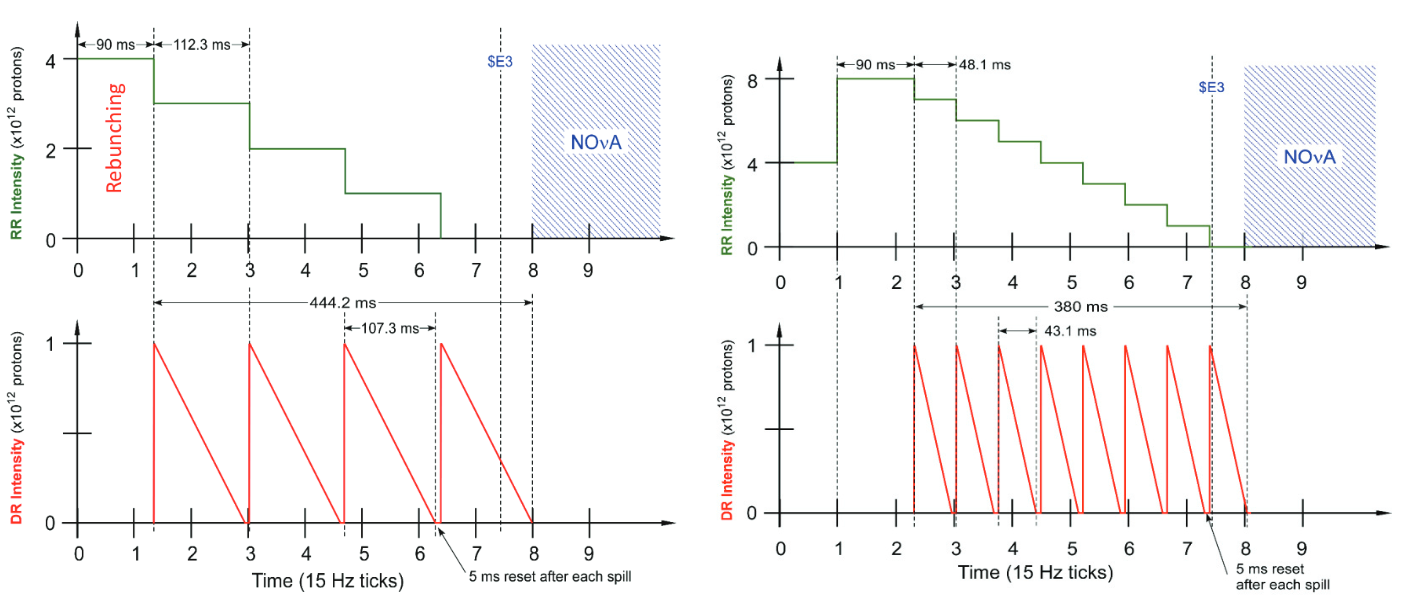
\includegraphics[width=0.9\linewidth]{figures/BeamStructure.png}
\caption{The beam structure as a function of time for the (left) low-intensity and (right) high-intensity modes. The recycler ring and delivery ring beam intensities are shown in green and red, respectively.}
\label{fig:beam}
\end{center}
\end{figure}

\subsection{Schedule and Data Taking Plan}
The Mu2e schedule derived from the Project WBS and the Ops WBS (June 2024) is displayed in Figure~\ref{fig:Mu2eRunPlan}. The major schedule milestones relevant to Mu2e Offline Computing are discussed below.
%
\begin{figure}[ht!]
\begin{center}
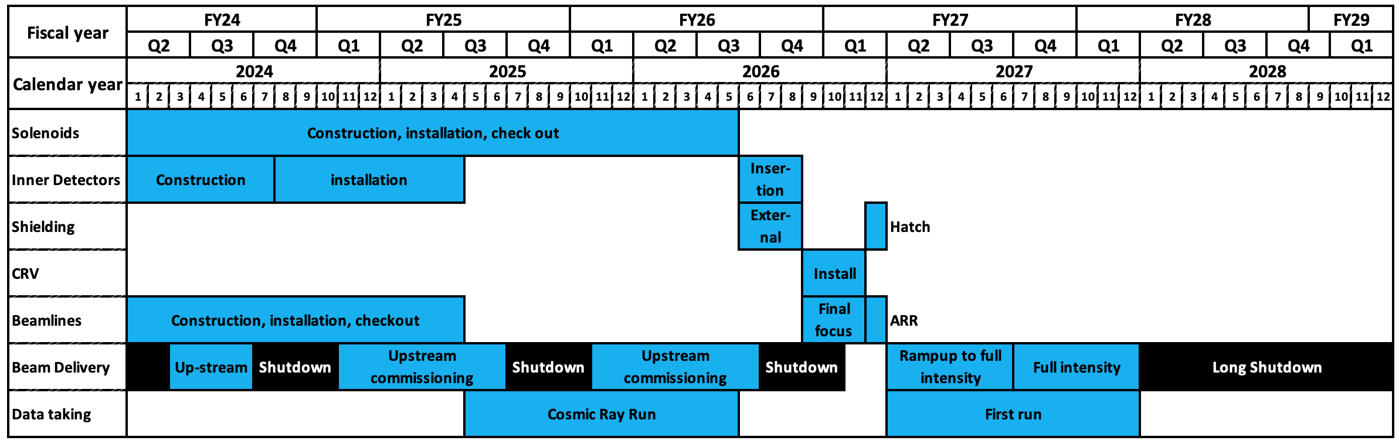
\includegraphics[width=0.9\linewidth]{figures/Mu2eTimeline2.png}
\caption{The Mu2e Schedule (June 2024)}
\label{fig:Mu2eRunPlan}
\end{center}
\end{figure}
%
{\bf Cosmic ray commissioning run - } The cosmic ray commissioning period will start in May 2025 and end with the achievement of the detector KPP, as described in Ref~\cite{docdb4665}. Immediately following the KPP, another cosmic ray run will start and continue until the detector is inserted into the magnet, currently scheduled for May 2026. During these periods, cosmic ray data will be recorded by the tracker, calorimeter, and a subset of the cosmic ray veto modules. The cosmic ray run will resume after the insertion of the tracker and calorimeter into the magnet, adding information from the full cosmic ray veto to the data stream. The data rates and associated storage needs should be relatively modest, but quick processing of the data will be required. 

In addition to supporting detector commissioning activities, offline computing will exercise the full processing chain: transferring data from the DAQ disks, performing the first reconstruction pass to derive calibration constants and producing data quality metrics, reprocessing data with updated calibration constants, and producing reduced datasets for analysis. The calibration and alignment procedures will be exercised with cosmic tracks and simulated events. Stress tests of the data logging and data processing with synthetic loads up to levels expected during normal data taking will be conducted, as well as stress tests of condition information delivery. Analysis tools and event displays will be further developed. Routine operation of many elements of offline computing will be demonstrated by the end of this phase. 

{\bf Beam commissioning - } The beam commissioning phase is expected to start in December 2026 with the full detector, including the stopping target and extinction monitors, at low beam intensity. Offline computing will commission the full data processing workflows with the complete detector in realistic beam conditions. Support to detector subsystem teams will be provided to refine algorithms, in particular calibration and alignment procedures, and continue the development of computing tools. Fast processing of raw detector data will be critical to provide detailed data quality monitoring and feedback to the detector sub-systems in a timely manner. At the end of this phase, offline computing will be ready for physics data taking.

{\bf Physics data taking - } Once stable beam conditions have been achieved, the DAQ configuration is optimized to record potential conversion electrons. A fraction of the trigger bandwidth will be allocated to dedicated calibration channels, and specific calibration runs will also be performed. Data are routinely processed by the first pass of offline reconstruction as soon as they have been transferred from the DAQ buffer disk, and data quality metrics are available within a few hours of data collection. Once calibration has been performed, the data are reprocessed with the updated calibration constants. Calibration data taken with specific configurations will require separate processing. This document assumes this configuration is used for the large majority of the data recorded and processed in the computing model.

{\bf Magnetic Field Mapping - } Precise reconstruction of tracks in Mu2e requires a detailed model of the DS magnetic field. A dedicated Mu2e operations team will oversee a detailed map of the Mu2e DS field using a custom device, and the conversion of those measurements into an Offline field model. Studies using a range of simulated coil displacements showed that a field model based on a calculation assuming the nominal DS coil positions meets the requirements of the Mu2e trigger~\cite{docdb46856}. Consequently, if the Mu2e operations schedule requires, the field map may be postponed until after run 1. Final quality track-based physics results will only be possible after the field model is complete and the data are reprocessed.


\subsection{Offline Computing challenges}

Mu2e offline computing faces several challenges, some of which are specific to Mu2e while others are shared by the HEP community.

\begin{itemize}

\item[] {\bf Simulation} - Mu2e is a precision experiment aiming to maintain a background level for the conversion search well below a single event. Given the expectation of $>10^{18}$ muons delivered, large samples of simulated events are needed to understand such low background levels. Directly simulating beam protons through the full detector response is prohibitively resource intensive in such quantities, so the simulation process is split into discrete stages, and resampling is used to reduce the computational cost. Managing simulation production and keeping track of information between these stages present non-trivial challenges. Integration of high-performance computing to speed up simulation campaigns introduces additional complications as well. These aspects are discussed in sections~\ref{sec:datahandling}, \ref{sec:dataProc}, and \ref{sec:simulation}.

\item[] {\bf Reconstruction and calibration} - To efficiently reject the DIO background, tracks must be reconstructed with a high degree of precision, and a high suppression of non-Gaussian tails. This requires accurate pattern recognition and track fitting, accurate calibration procedures based on dedicated data samples covering the full tracker region, and a precise magnetic field measurement. The unusual tracker geometry (un-instrumented inner region) presents other challenges as only segments of the track trajectories are recorded, and dedicated reconstruction algorithms are required to identify and reconstruct these topologies. Reconstruction and calibration are reviewed in sections~\ref{sec:reconstruction} and \ref{sec:calibration}.
 
\item[] {\bf Analysis} - Tools and reduced data formats need to be developed to enable efficient analysis of the data. Extraction of parameters of interest in the presence of many nuisance parameters remains a computationally intensive task and high-performance computing might prove beneficial to produce final results on time. Integration of machine learning techniques into a complex software ecosystem also requires substantial efforts to train models and support special data formats. Event displays also provide critical input to design analysis and extract physics results, and more generally operate the detector and develop algorithms. Sections~\ref{sec:analysis} and \ref{sec:display} focus on these topics.

\item[] {\bf System infrastructure} - A large suite of activities, common to many experiments, must be performed to ensure smooth and efficient computing operation. These include database design and operation, code development and management, documentation, and user support. In particular, the continuous technological progress and evolution of security requirements need frequent modifications to the overall computing system and associated workflows. Similarly, proper code management and documentation are essential to ensure the long-term success of the experiment. To reduce costs and the global environmental footprint, the computing architecture must be designed to efficiently use storage and CPU resources. These issues are examined in sections~\ref{sec:databases}, \ref{sec:codemanagement} and \ref{sec:datamngt}.

\item[] {\bf Documentation and training} - Besides optimizing workflows and algorithms, documentation and user training are essential components to improve coding practices and reduce nonessential data (re-)processing. Data quality monitoring also plays an important role in identifying and correcting issues as early as possible. Efficient On-boarding of new personnel also requires good training materials. Efforts in these domains are discussed in sections~\ref{sec:monitoring}, \ref{sec:documentation}, and \ref{sec:communication}.
\end{itemize} 